\documentclass[twoside]{book}

% Packages required by doxygen
\usepackage{calc}
\usepackage{doxygen}
\usepackage{graphicx}
\usepackage[utf8]{inputenc}
\usepackage{makeidx}
\usepackage{multicol}
\usepackage{multirow}
\usepackage{textcomp}
\usepackage[table]{xcolor}

% Font selection
\usepackage[T1]{fontenc}
\usepackage{mathptmx}
\usepackage[scaled=.90]{helvet}
\usepackage{courier}
\usepackage{amssymb}
\usepackage{sectsty}
\renewcommand{\familydefault}{\sfdefault}
\allsectionsfont{%
  \fontseries{bc}\selectfont%
  \color{darkgray}%
}
\renewcommand{\DoxyLabelFont}{%
  \fontseries{bc}\selectfont%
  \color{darkgray}%
}

% Page & text layout
\usepackage{geometry}
\geometry{%
  a4paper,%
  top=2.5cm,%
  bottom=2.5cm,%
  left=2.5cm,%
  right=2.5cm%
}
\tolerance=750
\hfuzz=15pt
\hbadness=750
\setlength{\emergencystretch}{15pt}
\setlength{\parindent}{0cm}
\setlength{\parskip}{0.2cm}
\makeatletter
\renewcommand{\paragraph}{%
  \@startsection{paragraph}{4}{0ex}{-1.0ex}{1.0ex}{%
    \normalfont\normalsize\bfseries\SS@parafont%
  }%
}
\renewcommand{\subparagraph}{%
  \@startsection{subparagraph}{5}{0ex}{-1.0ex}{1.0ex}{%
    \normalfont\normalsize\bfseries\SS@subparafont%
  }%
}
\makeatother

% Headers & footers
\usepackage{fancyhdr}
\pagestyle{fancyplain}
\fancyhead[LE]{\fancyplain{}{\bfseries\thepage}}
\fancyhead[CE]{\fancyplain{}{}}
\fancyhead[RE]{\fancyplain{}{\bfseries\leftmark}}
\fancyhead[LO]{\fancyplain{}{\bfseries\rightmark}}
\fancyhead[CO]{\fancyplain{}{}}
\fancyhead[RO]{\fancyplain{}{\bfseries\thepage}}
\fancyfoot[LE]{\fancyplain{}{}}
\fancyfoot[CE]{\fancyplain{}{}}
\fancyfoot[RE]{\fancyplain{}{\bfseries\scriptsize Generated on Mon Sep 19 2016 00\-:25\-:52 for P\-A01 by Doxygen }}
\fancyfoot[LO]{\fancyplain{}{\bfseries\scriptsize Generated on Mon Sep 19 2016 00\-:25\-:52 for P\-A01 by Doxygen }}
\fancyfoot[CO]{\fancyplain{}{}}
\fancyfoot[RO]{\fancyplain{}{}}
\renewcommand{\footrulewidth}{0.4pt}
\renewcommand{\chaptermark}[1]{%
  \markboth{#1}{}%
}
\renewcommand{\sectionmark}[1]{%
  \markright{\thesection\ #1}%
}

% Indices & bibliography
\usepackage{natbib}
\usepackage[titles]{tocloft}
\setcounter{tocdepth}{3}
\setcounter{secnumdepth}{5}
\makeindex

% Hyperlinks (required, but should be loaded last)
\usepackage{ifpdf}
\ifpdf
  \usepackage[pdftex,pagebackref=true]{hyperref}
\else
  \usepackage[ps2pdf,pagebackref=true]{hyperref}
\fi
\hypersetup{%
  colorlinks=true,%
  linkcolor=blue,%
  citecolor=blue,%
  unicode%
}

% Custom commands
\newcommand{\clearemptydoublepage}{%
  \newpage{\pagestyle{empty}\cleardoublepage}%
}


%===== C O N T E N T S =====

\begin{document}

% Titlepage & ToC
\hypersetup{pageanchor=false}
\pagenumbering{roman}
\begin{titlepage}
\vspace*{7cm}
\begin{center}%
{\Large P\-A01 }\\
\vspace*{1cm}
{\large Generated by Doxygen 1.8.6}\\
\vspace*{0.5cm}
{\small Mon Sep 19 2016 00:25:52}\\
\end{center}
\end{titlepage}
\clearemptydoublepage
\tableofcontents
\clearemptydoublepage
\pagenumbering{arabic}
\hypersetup{pageanchor=true}

%--- Begin generated contents ---
\chapter{Hierarchical Index}
\section{Class Hierarchy}
This inheritance list is sorted roughly, but not completely, alphabetically\+:\begin{DoxyCompactList}
\item \contentsline{section}{Event}{\pageref{struct_event}}{}
\item \contentsline{section}{Event\+Queue}{\pageref{class_event_queue}}{}
\begin{DoxyCompactList}
\item \contentsline{section}{A\+B\+Event\+Queue}{\pageref{class_a_b_event_queue}}{}
\item \contentsline{section}{L\+L\+Event\+Queue}{\pageref{class_l_l_event_queue}}{}
\end{DoxyCompactList}
\item \contentsline{section}{L\+L\+E\+Q\+Node}{\pageref{struct_l_l_e_q_node}}{}
\item \contentsline{section}{Teller\+Setup}{\pageref{class_teller_setup}}{}
\begin{DoxyCompactList}
\item \contentsline{section}{Teller\+Setup\+\_\+1\+QnT}{\pageref{class_teller_setup__1_qn_t}}{}
\item \contentsline{section}{Teller\+Setup\+\_\+n\+QnT}{\pageref{class_teller_setup__n_qn_t}}{}
\end{DoxyCompactList}
\item \contentsline{section}{Tickable}{\pageref{class_tickable}}{}
\begin{DoxyCompactList}
\item \contentsline{section}{Teller}{\pageref{class_teller}}{}
\item \contentsline{section}{Tickable\+Queue}{\pageref{class_tickable_queue}}{}
\end{DoxyCompactList}
\end{DoxyCompactList}

\chapter{Class Index}
\section{Class List}
Here are the classes, structs, unions and interfaces with brief descriptions\+:\begin{DoxyCompactList}
\item\contentsline{section}{\hyperlink{class_a_b_event_queue}{A\+B\+Event\+Queue} \\*An Array-\/\+Based \hyperlink{struct_event}{Event} Queue }{\pageref{class_a_b_event_queue}}{}
\item\contentsline{section}{\hyperlink{struct_event}{Event} }{\pageref{struct_event}}{}
\item\contentsline{section}{\hyperlink{class_event_queue}{Event\+Queue} }{\pageref{class_event_queue}}{}
\item\contentsline{section}{\hyperlink{struct_l_l_e_q_node}{L\+L\+E\+Q\+Node} \\*A node in an \hyperlink{class_l_l_event_queue}{L\+L\+Event\+Queue} }{\pageref{struct_l_l_e_q_node}}{}
\item\contentsline{section}{\hyperlink{class_l_l_event_queue}{L\+L\+Event\+Queue} \\*A Linked-\/\+List-\/\+Based \hyperlink{struct_event}{Event} Queue }{\pageref{class_l_l_event_queue}}{}
\item\contentsline{section}{\hyperlink{class_teller}{Teller} \\*Models a bank teller }{\pageref{class_teller}}{}
\item\contentsline{section}{\hyperlink{class_teller_setup}{Teller\+Setup} }{\pageref{class_teller_setup}}{}
\item\contentsline{section}{\hyperlink{class_teller_setup__1_qn_t}{Teller\+Setup\+\_\+1\+QnT} }{\pageref{class_teller_setup__1_qn_t}}{}
\item\contentsline{section}{\hyperlink{class_teller_setup__n_qn_t}{Teller\+Setup\+\_\+n\+QnT} }{\pageref{class_teller_setup__n_qn_t}}{}
\item\contentsline{section}{\hyperlink{class_tickable}{Tickable} \\*A \hyperlink{class_tickable}{Tickable} object }{\pageref{class_tickable}}{}
\item\contentsline{section}{\hyperlink{class_tickable_queue}{Tickable\+Queue} \\*An \hyperlink{class_event_queue}{Event\+Queue} wrapper that enables tick functionality }{\pageref{class_tickable_queue}}{}
\end{DoxyCompactList}

\chapter{File Index}
\section{File List}
Here is a list of all documented files with brief descriptions\+:\begin{DoxyCompactList}
\item\contentsline{section}{\hyperlink{PA02_8cpp}{P\+A02.\+cpp} \\*Implements the program entry point }{\pageref{PA02_8cpp}}{}
\end{DoxyCompactList}

\chapter{Class Documentation}
\hypertarget{class_linked_list}{\section{Linked\-List$<$ Item\-Type $>$ Class Template Reference}
\label{class_linked_list}\index{Linked\-List$<$ Item\-Type $>$@{Linked\-List$<$ Item\-Type $>$}}
}
Inheritance diagram for Linked\-List$<$ Item\-Type $>$\-:\begin{figure}[H]
\begin{center}
\leavevmode
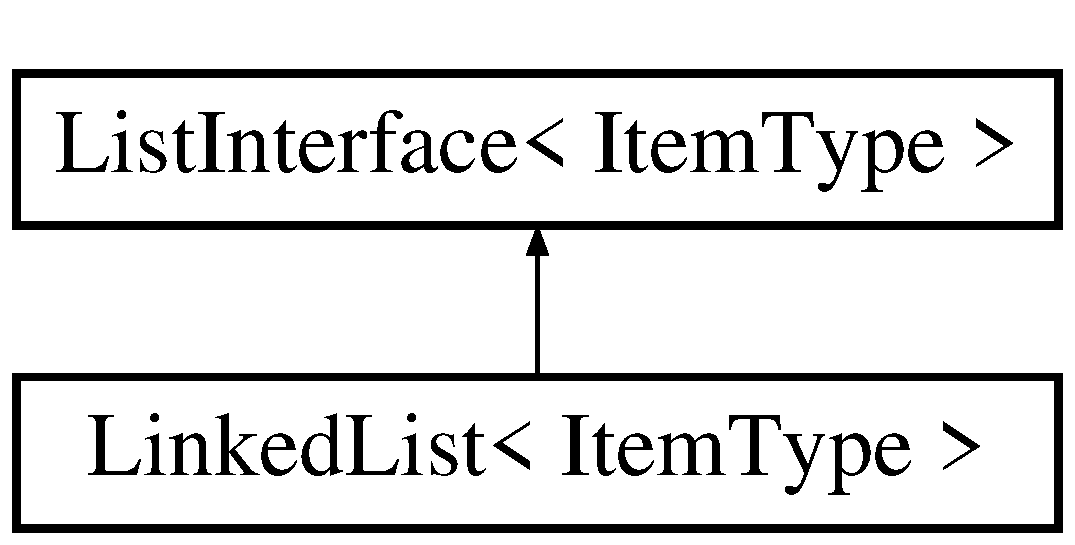
\includegraphics[height=2.000000cm]{class_linked_list}
\end{center}
\end{figure}
\subsection*{Public Member Functions}
\begin{DoxyCompactItemize}
\item 
\hypertarget{class_linked_list_adf8d8164e06b6d358a36df7e53e814ee}{\hyperlink{class_linked_list_adf8d8164e06b6d358a36df7e53e814ee}{Linked\-List} ()}\label{class_linked_list_adf8d8164e06b6d358a36df7e53e814ee}

\begin{DoxyCompactList}\small\item\em Constructs an empty linked list. \end{DoxyCompactList}\item 
\hyperlink{class_linked_list_a348f750d6770905429ca9c5068301baf}{Linked\-List} (const \hyperlink{class_linked_list}{Linked\-List}$<$ Item\-Type $>$ \&other)
\begin{DoxyCompactList}\small\item\em Copies the contents of another linked list. \end{DoxyCompactList}\item 
\hypertarget{class_linked_list_a66aee17d756fe0e002375897383c180b}{virtual \hyperlink{class_linked_list_a66aee17d756fe0e002375897383c180b}{$\sim$\-Linked\-List} ()}\label{class_linked_list_a66aee17d756fe0e002375897383c180b}

\begin{DoxyCompactList}\small\item\em Destructs the linked list object. \end{DoxyCompactList}\item 
bool \hyperlink{class_linked_list_adb17aed0ceacbbe1f247d235f491f0d5}{is\-Empty} () const 
\begin{DoxyCompactList}\small\item\em Sees whether this list is empty. \end{DoxyCompactList}\item 
int \hyperlink{class_linked_list_adae55d6b79235c816cb9e05027fd2e7a}{get\-Length} () const 
\item 
bool \hyperlink{class_linked_list_ae8a19375505e87e2e4fc0e9b5afe4d4d}{insert} (int new\-Position, const Item\-Type \&new\-Entry)
\item 
bool \hyperlink{class_linked_list_a16a02716b5b2efb6fb1e3d18721b53e4}{remove} (int position)
\item 
void \hyperlink{class_linked_list_a7d1d9cf83eef67b6c4d700a3cc5970e1}{clear} ()
\item 
Item\-Type \hyperlink{class_linked_list_a79f005e696c19f6ccf90d9d535afa999}{get\-Entry} (int position) const   throw (\-Precond\-Violated\-Except)
\begin{DoxyCompactList}\small\item\em Gets the entry found at the given position. \end{DoxyCompactList}\item 
void \hyperlink{class_linked_list_a3035f880c50e7d8f68e67c093d4607ca}{replace} (int position, const Item\-Type \&new\-Entry)  throw (\-Precond\-Violated\-Except)
\begin{DoxyCompactList}\small\item\em Replaces the entry at the given position with the specified new entry. \end{DoxyCompactList}\end{DoxyCompactItemize}


\subsection{Constructor \& Destructor Documentation}
\hypertarget{class_linked_list_a348f750d6770905429ca9c5068301baf}{\index{Linked\-List@{Linked\-List}!Linked\-List@{Linked\-List}}
\index{Linked\-List@{Linked\-List}!LinkedList@{Linked\-List}}
\subsubsection[{Linked\-List}]{\setlength{\rightskip}{0pt plus 5cm}template$<$class Item\-Type $>$ {\bf Linked\-List}$<$ Item\-Type $>$\-::{\bf Linked\-List} (
\begin{DoxyParamCaption}
\item[{const {\bf Linked\-List}$<$ Item\-Type $>$ \&}]{other}
\end{DoxyParamCaption}
)}}\label{class_linked_list_a348f750d6770905429ca9c5068301baf}


Copies the contents of another linked list. 


\begin{DoxyParams}{Parameters}
{\em other} & The linked list to copy. \\
\hline
\end{DoxyParams}


\subsection{Member Function Documentation}
\hypertarget{class_linked_list_a7d1d9cf83eef67b6c4d700a3cc5970e1}{\index{Linked\-List@{Linked\-List}!clear@{clear}}
\index{clear@{clear}!LinkedList@{Linked\-List}}
\subsubsection[{clear}]{\setlength{\rightskip}{0pt plus 5cm}template$<$class Item\-Type $>$ void {\bf Linked\-List}$<$ Item\-Type $>$\-::clear (
\begin{DoxyParamCaption}
{}
\end{DoxyParamCaption}
)\hspace{0.3cm}{\ttfamily [virtual]}}}\label{class_linked_list_a7d1d9cf83eef67b6c4d700a3cc5970e1}
Removes all entries from this list. \begin{DoxyPostcond}{Postcondition}
List contains no entries and the count of items is 0. 
\end{DoxyPostcond}


Implements \hyperlink{class_list_interface_adfda414908b645bdf19bcab8269168b7}{List\-Interface$<$ Item\-Type $>$}.

\hypertarget{class_linked_list_a79f005e696c19f6ccf90d9d535afa999}{\index{Linked\-List@{Linked\-List}!get\-Entry@{get\-Entry}}
\index{get\-Entry@{get\-Entry}!LinkedList@{Linked\-List}}
\subsubsection[{get\-Entry}]{\setlength{\rightskip}{0pt plus 5cm}template$<$class Item\-Type $>$ Item\-Type {\bf Linked\-List}$<$ Item\-Type $>$\-::get\-Entry (
\begin{DoxyParamCaption}
\item[{int}]{position}
\end{DoxyParamCaption}
) const throw  {\bf Precond\-Violated\-Except}) \hspace{0.3cm}{\ttfamily [virtual]}}}\label{class_linked_list_a79f005e696c19f6ccf90d9d535afa999}


Gets the entry found at the given position. 

Throws \hyperlink{class_precond_violated_except}{Precond\-Violated\-Except} on precondition violation. \begin{DoxyPrecond}{Precondition}
\hyperlink{class_linked_list_adae55d6b79235c816cb9e05027fd2e7a}{get\-Length()} != 0, 1 $<$= position $<$= \hyperlink{class_linked_list_adae55d6b79235c816cb9e05027fd2e7a}{get\-Length()} 
\end{DoxyPrecond}

\begin{DoxyParams}{Parameters}
{\em position} & The position of the entry to return. \\
\hline
\end{DoxyParams}
\begin{DoxyReturn}{Returns}
The entry at the specified position. 
\end{DoxyReturn}


Implements \hyperlink{class_list_interface_a86987f69e5056d287212ede41db1956a}{List\-Interface$<$ Item\-Type $>$}.

\hypertarget{class_linked_list_adae55d6b79235c816cb9e05027fd2e7a}{\index{Linked\-List@{Linked\-List}!get\-Length@{get\-Length}}
\index{get\-Length@{get\-Length}!LinkedList@{Linked\-List}}
\subsubsection[{get\-Length}]{\setlength{\rightskip}{0pt plus 5cm}template$<$class Item\-Type $>$ int {\bf Linked\-List}$<$ Item\-Type $>$\-::get\-Length (
\begin{DoxyParamCaption}
{}
\end{DoxyParamCaption}
) const\hspace{0.3cm}{\ttfamily [virtual]}}}\label{class_linked_list_adae55d6b79235c816cb9e05027fd2e7a}
Gets the current number of entries in this list. \begin{DoxyReturn}{Returns}
The integer number of entries currently in the list. 
\end{DoxyReturn}


Implements \hyperlink{class_list_interface_afc85695d4137f1e29ff02e179c9f3221}{List\-Interface$<$ Item\-Type $>$}.

\hypertarget{class_linked_list_ae8a19375505e87e2e4fc0e9b5afe4d4d}{\index{Linked\-List@{Linked\-List}!insert@{insert}}
\index{insert@{insert}!LinkedList@{Linked\-List}}
\subsubsection[{insert}]{\setlength{\rightskip}{0pt plus 5cm}template$<$class Item\-Type $>$ bool {\bf Linked\-List}$<$ Item\-Type $>$\-::insert (
\begin{DoxyParamCaption}
\item[{int}]{new\-Position, }
\item[{const Item\-Type \&}]{new\-Entry}
\end{DoxyParamCaption}
)\hspace{0.3cm}{\ttfamily [virtual]}}}\label{class_linked_list_ae8a19375505e87e2e4fc0e9b5afe4d4d}
Inserts an entry into this list at a given position. \begin{DoxyPrecond}{Precondition}
None. 
\end{DoxyPrecond}
\begin{DoxyPostcond}{Postcondition}
If 1 $<$= position $<$= \hyperlink{class_linked_list_adae55d6b79235c816cb9e05027fd2e7a}{get\-Length()} + 1 and the insertion is successful, new\-Entry is at the given position in the list, other entries are renumbered accordingly, and the returned value is true. 
\end{DoxyPostcond}

\begin{DoxyParams}{Parameters}
{\em new\-Position} & The list position at which to insert new\-Entry. \\
\hline
{\em new\-Entry} & The entry to insert into the list. \\
\hline
\end{DoxyParams}
\begin{DoxyReturn}{Returns}
True if insertion is successful, or false if not. 
\end{DoxyReturn}


Implements \hyperlink{class_list_interface_a5b2f86954a86172699a3495982c38e77}{List\-Interface$<$ Item\-Type $>$}.

\hypertarget{class_linked_list_adb17aed0ceacbbe1f247d235f491f0d5}{\index{Linked\-List@{Linked\-List}!is\-Empty@{is\-Empty}}
\index{is\-Empty@{is\-Empty}!LinkedList@{Linked\-List}}
\subsubsection[{is\-Empty}]{\setlength{\rightskip}{0pt plus 5cm}template$<$class Item\-Type $>$ bool {\bf Linked\-List}$<$ Item\-Type $>$\-::is\-Empty (
\begin{DoxyParamCaption}
{}
\end{DoxyParamCaption}
) const\hspace{0.3cm}{\ttfamily [virtual]}}}\label{class_linked_list_adb17aed0ceacbbe1f247d235f491f0d5}


Sees whether this list is empty. 

\begin{DoxyReturn}{Returns}
True if the list is empty, false othersise. 
\end{DoxyReturn}


Implements \hyperlink{class_list_interface_a924f91e7f81d7dcd3fda79bbcc671394}{List\-Interface$<$ Item\-Type $>$}.

\hypertarget{class_linked_list_a16a02716b5b2efb6fb1e3d18721b53e4}{\index{Linked\-List@{Linked\-List}!remove@{remove}}
\index{remove@{remove}!LinkedList@{Linked\-List}}
\subsubsection[{remove}]{\setlength{\rightskip}{0pt plus 5cm}template$<$class Item\-Type $>$ bool {\bf Linked\-List}$<$ Item\-Type $>$\-::remove (
\begin{DoxyParamCaption}
\item[{int}]{position}
\end{DoxyParamCaption}
)\hspace{0.3cm}{\ttfamily [virtual]}}}\label{class_linked_list_a16a02716b5b2efb6fb1e3d18721b53e4}
Removes the entry at a given position from this list. \begin{DoxyPrecond}{Precondition}
None. 
\end{DoxyPrecond}
\begin{DoxyPostcond}{Postcondition}
If 1 $<$= position $<$= \hyperlink{class_linked_list_adae55d6b79235c816cb9e05027fd2e7a}{get\-Length()} and the removal is successful, the entry at the given position in the list is removed, other items are renumbered accordingly, and the returned value is true. 
\end{DoxyPostcond}

\begin{DoxyParams}{Parameters}
{\em position} & The list position of the entry to remove. \\
\hline
\end{DoxyParams}
\begin{DoxyReturn}{Returns}
True if removal is successful, or false if not. 
\end{DoxyReturn}


Implements \hyperlink{class_list_interface_a5543002ec0d64bd2a63f3732f437af65}{List\-Interface$<$ Item\-Type $>$}.

\hypertarget{class_linked_list_a3035f880c50e7d8f68e67c093d4607ca}{\index{Linked\-List@{Linked\-List}!replace@{replace}}
\index{replace@{replace}!LinkedList@{Linked\-List}}
\subsubsection[{replace}]{\setlength{\rightskip}{0pt plus 5cm}template$<$class Item\-Type $>$ void {\bf Linked\-List}$<$ Item\-Type $>$\-::replace (
\begin{DoxyParamCaption}
\item[{int}]{position, }
\item[{const Item\-Type \&}]{new\-Entry}
\end{DoxyParamCaption}
) throw  {\bf Precond\-Violated\-Except}) \hspace{0.3cm}{\ttfamily [virtual]}}}\label{class_linked_list_a3035f880c50e7d8f68e67c093d4607ca}


Replaces the entry at the given position with the specified new entry. 

Throws \hyperlink{class_precond_violated_except}{Precond\-Violated\-Except} on precondition violation. \begin{DoxyPrecond}{Precondition}
\hyperlink{class_linked_list_adae55d6b79235c816cb9e05027fd2e7a}{get\-Length()} != 0, 1 $<$= position $<$= \hyperlink{class_linked_list_adae55d6b79235c816cb9e05027fd2e7a}{get\-Length()} 
\end{DoxyPrecond}
\begin{DoxyPostcond}{Postcondition}
The entry at the given position has been replaced. 
\end{DoxyPostcond}

\begin{DoxyParams}{Parameters}
{\em position} & The position of the entry to replace. \\
\hline
{\em new\-Entry} & The new value of the entry. \\
\hline
\end{DoxyParams}


Implements \hyperlink{class_list_interface_aae877a56b7b9f5f526c37a00e234fad1}{List\-Interface$<$ Item\-Type $>$}.



The documentation for this class was generated from the following files\-:\begin{DoxyCompactItemize}
\item 
\hyperlink{_linked_list_8h}{Linked\-List.\-h}\item 
\hyperlink{_linked_list_8cpp}{Linked\-List.\-cpp}\end{DoxyCompactItemize}

\hypertarget{class_list_interface}{\section{List\-Interface$<$ Item\-Type $>$ Class Template Reference}
\label{class_list_interface}\index{List\-Interface$<$ Item\-Type $>$@{List\-Interface$<$ Item\-Type $>$}}
}
Inheritance diagram for List\-Interface$<$ Item\-Type $>$\-:\begin{figure}[H]
\begin{center}
\leavevmode
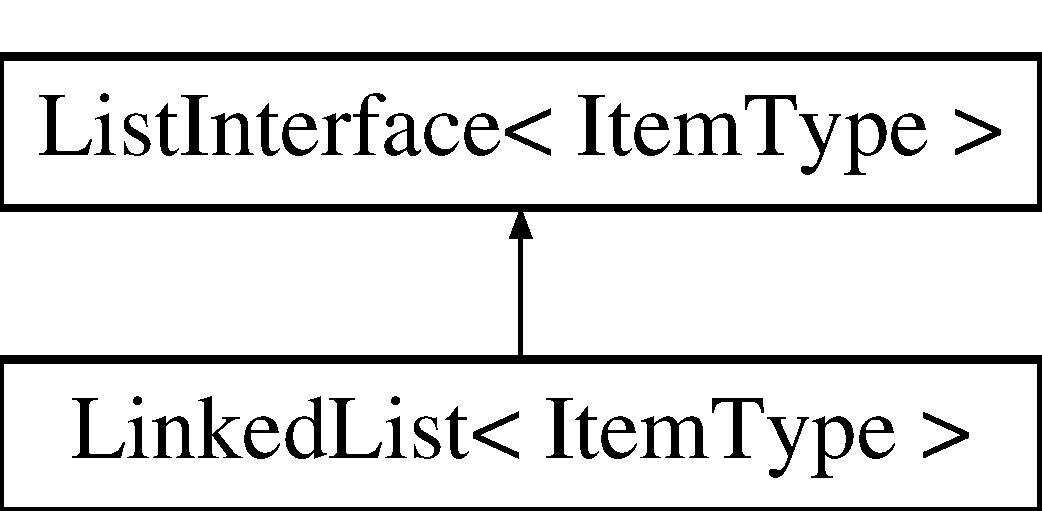
\includegraphics[height=2.000000cm]{class_list_interface}
\end{center}
\end{figure}
\subsection*{Public Member Functions}
\begin{DoxyCompactItemize}
\item 
virtual bool \hyperlink{class_list_interface_a924f91e7f81d7dcd3fda79bbcc671394}{is\-Empty} () const =0
\item 
virtual int \hyperlink{class_list_interface_afc85695d4137f1e29ff02e179c9f3221}{get\-Length} () const =0
\item 
virtual bool \hyperlink{class_list_interface_a5b2f86954a86172699a3495982c38e77}{insert} (int new\-Position, const Item\-Type \&new\-Entry)=0
\item 
virtual bool \hyperlink{class_list_interface_a5543002ec0d64bd2a63f3732f437af65}{remove} (int position)=0
\item 
virtual void \hyperlink{class_list_interface_adfda414908b645bdf19bcab8269168b7}{clear} ()=0
\item 
virtual Item\-Type \hyperlink{class_list_interface_a86987f69e5056d287212ede41db1956a}{get\-Entry} (int position) const =0
\item 
virtual void \hyperlink{class_list_interface_aae877a56b7b9f5f526c37a00e234fad1}{replace} (int position, const Item\-Type \&new\-Entry)=0
\end{DoxyCompactItemize}


\subsection{Member Function Documentation}
\hypertarget{class_list_interface_adfda414908b645bdf19bcab8269168b7}{\index{List\-Interface@{List\-Interface}!clear@{clear}}
\index{clear@{clear}!ListInterface@{List\-Interface}}
\subsubsection[{clear}]{\setlength{\rightskip}{0pt plus 5cm}template$<$class Item\-Type $>$ virtual void {\bf List\-Interface}$<$ Item\-Type $>$\-::clear (
\begin{DoxyParamCaption}
{}
\end{DoxyParamCaption}
)\hspace{0.3cm}{\ttfamily [pure virtual]}}}\label{class_list_interface_adfda414908b645bdf19bcab8269168b7}
Removes all entries from this list. \begin{DoxyPostcond}{Postcondition}
List contains no entries and the count of items is 0. 
\end{DoxyPostcond}


Implemented in \hyperlink{class_linked_list_a7d1d9cf83eef67b6c4d700a3cc5970e1}{Linked\-List$<$ Item\-Type $>$}.

\hypertarget{class_list_interface_a86987f69e5056d287212ede41db1956a}{\index{List\-Interface@{List\-Interface}!get\-Entry@{get\-Entry}}
\index{get\-Entry@{get\-Entry}!ListInterface@{List\-Interface}}
\subsubsection[{get\-Entry}]{\setlength{\rightskip}{0pt plus 5cm}template$<$class Item\-Type $>$ virtual Item\-Type {\bf List\-Interface}$<$ Item\-Type $>$\-::get\-Entry (
\begin{DoxyParamCaption}
\item[{int}]{position}
\end{DoxyParamCaption}
) const\hspace{0.3cm}{\ttfamily [pure virtual]}}}\label{class_list_interface_a86987f69e5056d287212ede41db1956a}
Gets the entry at the given position in this list. \begin{DoxyPrecond}{Precondition}
1 $<$= position $<$= \hyperlink{class_list_interface_afc85695d4137f1e29ff02e179c9f3221}{get\-Length()}. 
\end{DoxyPrecond}
\begin{DoxyPostcond}{Postcondition}
The desired entry has been returned. 
\end{DoxyPostcond}

\begin{DoxyParams}{Parameters}
{\em position} & The list position of the desired entry. \\
\hline
\end{DoxyParams}
\begin{DoxyReturn}{Returns}
The entry at the given position. 
\end{DoxyReturn}


Implemented in \hyperlink{class_linked_list_a79f005e696c19f6ccf90d9d535afa999}{Linked\-List$<$ Item\-Type $>$}.

\hypertarget{class_list_interface_afc85695d4137f1e29ff02e179c9f3221}{\index{List\-Interface@{List\-Interface}!get\-Length@{get\-Length}}
\index{get\-Length@{get\-Length}!ListInterface@{List\-Interface}}
\subsubsection[{get\-Length}]{\setlength{\rightskip}{0pt plus 5cm}template$<$class Item\-Type $>$ virtual int {\bf List\-Interface}$<$ Item\-Type $>$\-::get\-Length (
\begin{DoxyParamCaption}
{}
\end{DoxyParamCaption}
) const\hspace{0.3cm}{\ttfamily [pure virtual]}}}\label{class_list_interface_afc85695d4137f1e29ff02e179c9f3221}
Gets the current number of entries in this list. \begin{DoxyReturn}{Returns}
The integer number of entries currently in the list. 
\end{DoxyReturn}


Implemented in \hyperlink{class_linked_list_adae55d6b79235c816cb9e05027fd2e7a}{Linked\-List$<$ Item\-Type $>$}.

\hypertarget{class_list_interface_a5b2f86954a86172699a3495982c38e77}{\index{List\-Interface@{List\-Interface}!insert@{insert}}
\index{insert@{insert}!ListInterface@{List\-Interface}}
\subsubsection[{insert}]{\setlength{\rightskip}{0pt plus 5cm}template$<$class Item\-Type $>$ virtual bool {\bf List\-Interface}$<$ Item\-Type $>$\-::insert (
\begin{DoxyParamCaption}
\item[{int}]{new\-Position, }
\item[{const Item\-Type \&}]{new\-Entry}
\end{DoxyParamCaption}
)\hspace{0.3cm}{\ttfamily [pure virtual]}}}\label{class_list_interface_a5b2f86954a86172699a3495982c38e77}
Inserts an entry into this list at a given position. \begin{DoxyPrecond}{Precondition}
None. 
\end{DoxyPrecond}
\begin{DoxyPostcond}{Postcondition}
If 1 $<$= position $<$= \hyperlink{class_list_interface_afc85695d4137f1e29ff02e179c9f3221}{get\-Length()} + 1 and the insertion is successful, new\-Entry is at the given position in the list, other entries are renumbered accordingly, and the returned value is true. 
\end{DoxyPostcond}

\begin{DoxyParams}{Parameters}
{\em new\-Position} & The list position at which to insert new\-Entry. \\
\hline
{\em new\-Entry} & The entry to insert into the list. \\
\hline
\end{DoxyParams}
\begin{DoxyReturn}{Returns}
True if insertion is successful, or false if not. 
\end{DoxyReturn}


Implemented in \hyperlink{class_linked_list_ae8a19375505e87e2e4fc0e9b5afe4d4d}{Linked\-List$<$ Item\-Type $>$}.

\hypertarget{class_list_interface_a924f91e7f81d7dcd3fda79bbcc671394}{\index{List\-Interface@{List\-Interface}!is\-Empty@{is\-Empty}}
\index{is\-Empty@{is\-Empty}!ListInterface@{List\-Interface}}
\subsubsection[{is\-Empty}]{\setlength{\rightskip}{0pt plus 5cm}template$<$class Item\-Type $>$ virtual bool {\bf List\-Interface}$<$ Item\-Type $>$\-::is\-Empty (
\begin{DoxyParamCaption}
{}
\end{DoxyParamCaption}
) const\hspace{0.3cm}{\ttfamily [pure virtual]}}}\label{class_list_interface_a924f91e7f81d7dcd3fda79bbcc671394}
Sees whether this list is empty. \begin{DoxyReturn}{Returns}
True if the list is empty; otherwise returns false. 
\end{DoxyReturn}


Implemented in \hyperlink{class_linked_list_adb17aed0ceacbbe1f247d235f491f0d5}{Linked\-List$<$ Item\-Type $>$}.

\hypertarget{class_list_interface_a5543002ec0d64bd2a63f3732f437af65}{\index{List\-Interface@{List\-Interface}!remove@{remove}}
\index{remove@{remove}!ListInterface@{List\-Interface}}
\subsubsection[{remove}]{\setlength{\rightskip}{0pt plus 5cm}template$<$class Item\-Type $>$ virtual bool {\bf List\-Interface}$<$ Item\-Type $>$\-::remove (
\begin{DoxyParamCaption}
\item[{int}]{position}
\end{DoxyParamCaption}
)\hspace{0.3cm}{\ttfamily [pure virtual]}}}\label{class_list_interface_a5543002ec0d64bd2a63f3732f437af65}
Removes the entry at a given position from this list. \begin{DoxyPrecond}{Precondition}
None. 
\end{DoxyPrecond}
\begin{DoxyPostcond}{Postcondition}
If 1 $<$= position $<$= \hyperlink{class_list_interface_afc85695d4137f1e29ff02e179c9f3221}{get\-Length()} and the removal is successful, the entry at the given position in the list is removed, other items are renumbered accordingly, and the returned value is true. 
\end{DoxyPostcond}

\begin{DoxyParams}{Parameters}
{\em position} & The list position of the entry to remove. \\
\hline
\end{DoxyParams}
\begin{DoxyReturn}{Returns}
True if removal is successful, or false if not. 
\end{DoxyReturn}


Implemented in \hyperlink{class_linked_list_a16a02716b5b2efb6fb1e3d18721b53e4}{Linked\-List$<$ Item\-Type $>$}.

\hypertarget{class_list_interface_aae877a56b7b9f5f526c37a00e234fad1}{\index{List\-Interface@{List\-Interface}!replace@{replace}}
\index{replace@{replace}!ListInterface@{List\-Interface}}
\subsubsection[{replace}]{\setlength{\rightskip}{0pt plus 5cm}template$<$class Item\-Type $>$ virtual void {\bf List\-Interface}$<$ Item\-Type $>$\-::replace (
\begin{DoxyParamCaption}
\item[{int}]{position, }
\item[{const Item\-Type \&}]{new\-Entry}
\end{DoxyParamCaption}
)\hspace{0.3cm}{\ttfamily [pure virtual]}}}\label{class_list_interface_aae877a56b7b9f5f526c37a00e234fad1}
Replaces the entry at the given position in this list. \begin{DoxyPrecond}{Precondition}
1 $<$= position $<$= \hyperlink{class_list_interface_afc85695d4137f1e29ff02e179c9f3221}{get\-Length()}. 
\end{DoxyPrecond}
\begin{DoxyPostcond}{Postcondition}
The entry at the given position is new\-Entry. 
\end{DoxyPostcond}

\begin{DoxyParams}{Parameters}
{\em position} & The list position of the entry to replace. \\
\hline
{\em new\-Entry} & The replacement entry. \\
\hline
\end{DoxyParams}


Implemented in \hyperlink{class_linked_list_a3035f880c50e7d8f68e67c093d4607ca}{Linked\-List$<$ Item\-Type $>$}.



The documentation for this class was generated from the following file\-:\begin{DoxyCompactItemize}
\item 
\hyperlink{_list_interface_8h}{List\-Interface.\-h}\end{DoxyCompactItemize}

\hypertarget{class_node}{\section{Node$<$ Item\-Type $>$ Class Template Reference}
\label{class_node}\index{Node$<$ Item\-Type $>$@{Node$<$ Item\-Type $>$}}
}
\subsection*{Public Member Functions}
\begin{DoxyCompactItemize}
\item 
\hypertarget{class_node_a627e94f4fba0e73c546e0fb2a7266f36}{\hyperlink{class_node_a627e94f4fba0e73c546e0fb2a7266f36}{Node} ()}\label{class_node_a627e94f4fba0e73c546e0fb2a7266f36}

\begin{DoxyCompactList}\small\item\em Construct an empty node. \end{DoxyCompactList}\item 
\hyperlink{class_node_a0288598fcb0244739ce95099c26250ae}{Node} (const Item\-Type \&an\-Item)
\begin{DoxyCompactList}\small\item\em Construct a node containing the given item. \end{DoxyCompactList}\item 
\hyperlink{class_node_adf98d3f9b7227622cb5a0fdd7e8f0b18}{Node} (const Item\-Type \&an\-Item, \hyperlink{class_node}{Node}$<$ Item\-Type $>$ $\ast$next\-Node\-Ptr)
\begin{DoxyCompactList}\small\item\em Construct a node containing the given item and pointing to the given next node. \end{DoxyCompactList}\item 
void \hyperlink{class_node_ab4ceecdecc5df799011de486b9f54974}{set\-Item} (const Item\-Type \&an\-Item)
\begin{DoxyCompactList}\small\item\em Set the contained item to the given item. \end{DoxyCompactList}\item 
void \hyperlink{class_node_a01c1a66d4e39f5b149e090413deb4633}{set\-Next} (\hyperlink{class_node}{Node}$<$ Item\-Type $>$ $\ast$next\-Node\-Ptr)
\begin{DoxyCompactList}\small\item\em Set the next node to the given node. \end{DoxyCompactList}\item 
Item\-Type \hyperlink{class_node_a4e5519463291a0c1570014f4ee5ca130}{get\-Item} () const 
\begin{DoxyCompactList}\small\item\em Get the item contained by this node. \end{DoxyCompactList}\item 
\hypertarget{class_node_a44fbda8e8d17a37e8203434c2909ea07}{\hyperlink{class_node}{Node}$<$ Item\-Type $>$ $\ast$ {\bfseries get\-Next} () const }\label{class_node_a44fbda8e8d17a37e8203434c2909ea07}

\end{DoxyCompactItemize}


\subsection{Constructor \& Destructor Documentation}
\hypertarget{class_node_a0288598fcb0244739ce95099c26250ae}{\index{Node@{Node}!Node@{Node}}
\index{Node@{Node}!Node@{Node}}
\subsubsection[{Node}]{\setlength{\rightskip}{0pt plus 5cm}template$<$class Item\-Type $>$ {\bf Node}$<$ Item\-Type $>$\-::{\bf Node} (
\begin{DoxyParamCaption}
\item[{const Item\-Type \&}]{an\-Item}
\end{DoxyParamCaption}
)}}\label{class_node_a0288598fcb0244739ce95099c26250ae}


Construct a node containing the given item. 

\begin{DoxyPostcond}{Postcondition}
The node will contain the given item. 
\end{DoxyPostcond}

\begin{DoxyParams}{Parameters}
{\em an\-Item} & The item to contain. \\
\hline
\end{DoxyParams}
\hypertarget{class_node_adf98d3f9b7227622cb5a0fdd7e8f0b18}{\index{Node@{Node}!Node@{Node}}
\index{Node@{Node}!Node@{Node}}
\subsubsection[{Node}]{\setlength{\rightskip}{0pt plus 5cm}template$<$class Item\-Type $>$ {\bf Node}$<$ Item\-Type $>$\-::{\bf Node} (
\begin{DoxyParamCaption}
\item[{const Item\-Type \&}]{an\-Item, }
\item[{{\bf Node}$<$ Item\-Type $>$ $\ast$}]{next\-Node\-Ptr}
\end{DoxyParamCaption}
)}}\label{class_node_adf98d3f9b7227622cb5a0fdd7e8f0b18}


Construct a node containing the given item and pointing to the given next node. 

\begin{DoxyPostcond}{Postcondition}
The node will contain the given item and will point to the given next node. 
\end{DoxyPostcond}

\begin{DoxyParams}{Parameters}
{\em an\-Item} & The item to contain. \\
\hline
{\em next\-Node\-Ptr} & The pointer to the next node. \\
\hline
\end{DoxyParams}


\subsection{Member Function Documentation}
\hypertarget{class_node_a4e5519463291a0c1570014f4ee5ca130}{\index{Node@{Node}!get\-Item@{get\-Item}}
\index{get\-Item@{get\-Item}!Node@{Node}}
\subsubsection[{get\-Item}]{\setlength{\rightskip}{0pt plus 5cm}template$<$class Item\-Type $>$ Item\-Type {\bf Node}$<$ Item\-Type $>$\-::get\-Item (
\begin{DoxyParamCaption}
{}
\end{DoxyParamCaption}
) const}}\label{class_node_a4e5519463291a0c1570014f4ee5ca130}


Get the item contained by this node. 

\begin{DoxyReturn}{Returns}
The item contained by this node. 
\end{DoxyReturn}
\hypertarget{class_node_ab4ceecdecc5df799011de486b9f54974}{\index{Node@{Node}!set\-Item@{set\-Item}}
\index{set\-Item@{set\-Item}!Node@{Node}}
\subsubsection[{set\-Item}]{\setlength{\rightskip}{0pt plus 5cm}template$<$class Item\-Type $>$ void {\bf Node}$<$ Item\-Type $>$\-::set\-Item (
\begin{DoxyParamCaption}
\item[{const Item\-Type \&}]{an\-Item}
\end{DoxyParamCaption}
)}}\label{class_node_ab4ceecdecc5df799011de486b9f54974}


Set the contained item to the given item. 

\begin{DoxyPostcond}{Postcondition}
The item will have been set to the given item. 
\end{DoxyPostcond}

\begin{DoxyParams}{Parameters}
{\em an\-Item} & The new item to be contained. \\
\hline
\end{DoxyParams}
\hypertarget{class_node_a01c1a66d4e39f5b149e090413deb4633}{\index{Node@{Node}!set\-Next@{set\-Next}}
\index{set\-Next@{set\-Next}!Node@{Node}}
\subsubsection[{set\-Next}]{\setlength{\rightskip}{0pt plus 5cm}template$<$class Item\-Type $>$ void {\bf Node}$<$ Item\-Type $>$\-::set\-Next (
\begin{DoxyParamCaption}
\item[{{\bf Node}$<$ Item\-Type $>$ $\ast$}]{next\-Node\-Ptr}
\end{DoxyParamCaption}
)}}\label{class_node_a01c1a66d4e39f5b149e090413deb4633}


Set the next node to the given node. 

\begin{DoxyPostcond}{Postcondition}
This node will point to the given next node. 
\end{DoxyPostcond}

\begin{DoxyParams}{Parameters}
{\em next\-Node\-Ptr} & The pointer to the next node. \\
\hline
\end{DoxyParams}


The documentation for this class was generated from the following files\-:\begin{DoxyCompactItemize}
\item 
\hyperlink{_node_8h}{Node.\-h}\item 
\hyperlink{_node_8cpp}{Node.\-cpp}\end{DoxyCompactItemize}

\hypertarget{class_precond_violated_except}{\section{Precond\-Violated\-Except Class Reference}
\label{class_precond_violated_except}\index{Precond\-Violated\-Except@{Precond\-Violated\-Except}}
}
Inheritance diagram for Precond\-Violated\-Except\-:\begin{figure}[H]
\begin{center}
\leavevmode
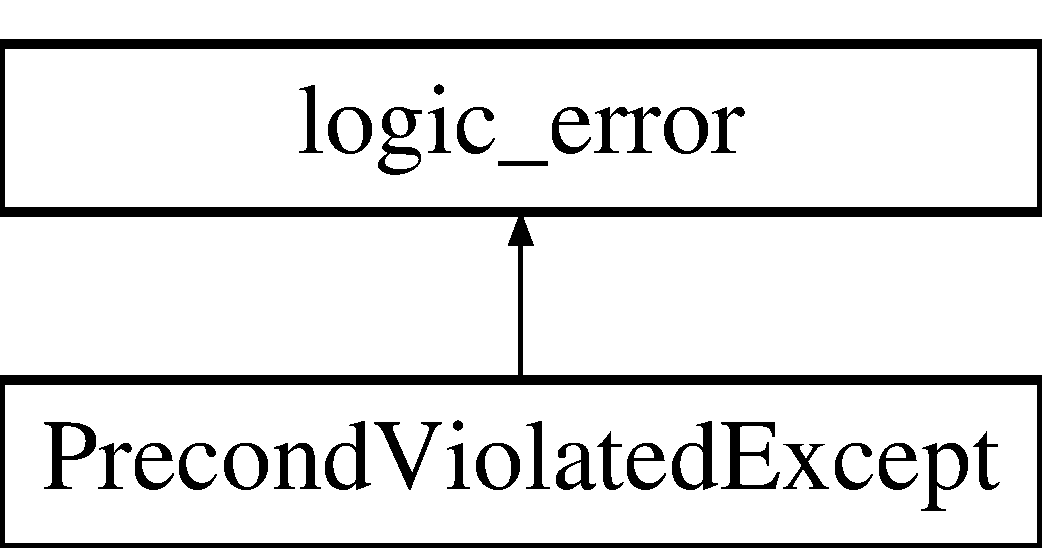
\includegraphics[height=2.000000cm]{class_precond_violated_except}
\end{center}
\end{figure}
\subsection*{Public Member Functions}
\begin{DoxyCompactItemize}
\item 
\hyperlink{class_precond_violated_except_a13c9075198f291ffc9a74c0c9b787ecf}{Precond\-Violated\-Except} (const std\-::string \&message=\char`\"{}\char`\"{})
\begin{DoxyCompactList}\small\item\em Construct a \hyperlink{class_precond_violated_except}{Precond\-Violated\-Except} with the given message. \end{DoxyCompactList}\end{DoxyCompactItemize}


\subsection{Constructor \& Destructor Documentation}
\hypertarget{class_precond_violated_except_a13c9075198f291ffc9a74c0c9b787ecf}{\index{Precond\-Violated\-Except@{Precond\-Violated\-Except}!Precond\-Violated\-Except@{Precond\-Violated\-Except}}
\index{Precond\-Violated\-Except@{Precond\-Violated\-Except}!PrecondViolatedExcept@{Precond\-Violated\-Except}}
\subsubsection[{Precond\-Violated\-Except}]{\setlength{\rightskip}{0pt plus 5cm}Precond\-Violated\-Except\-::\-Precond\-Violated\-Except (
\begin{DoxyParamCaption}
\item[{const std\-::string \&}]{message = {\ttfamily \char`\"{}\char`\"{}}}
\end{DoxyParamCaption}
)}}\label{class_precond_violated_except_a13c9075198f291ffc9a74c0c9b787ecf}


Construct a \hyperlink{class_precond_violated_except}{Precond\-Violated\-Except} with the given message. 

\begin{DoxyPostcond}{Postcondition}
The constructed object's message will match the one specified by the message parameter. 
\end{DoxyPostcond}

\begin{DoxyParams}{Parameters}
{\em message} & The message to be held. \\
\hline
\end{DoxyParams}


The documentation for this class was generated from the following files\-:\begin{DoxyCompactItemize}
\item 
\hyperlink{_precond_violated_except_8h}{Precond\-Violated\-Except.\-h}\item 
\hyperlink{_precond_violated_except_8cpp}{Precond\-Violated\-Except.\-cpp}\end{DoxyCompactItemize}

\chapter{File Documentation}
\hypertarget{_linked_list_8cpp}{\section{Linked\-List.\-cpp File Reference}
\label{_linked_list_8cpp}\index{Linked\-List.\-cpp@{Linked\-List.\-cpp}}
}


Implementation file for the \hyperlink{class_linked_list}{Linked\-List} data type.  


{\ttfamily \#include \char`\"{}Linked\-List.\-h\char`\"{}}\\*


\subsection{Detailed Description}
Implementation file for the \hyperlink{class_linked_list}{Linked\-List} data type. \begin{DoxyAuthor}{Author}
Matthew Bauer
\end{DoxyAuthor}
Implements the \hyperlink{class_linked_list}{Linked\-List} data type  Adapted from/inspired by \char`\"{}\-Data Abstractions \& Problem Solving
    with C++\char`\"{} Seventh Edition by Frank M. Carrano and Timothy M. Henry. 
\hypertarget{_linked_list_8h}{\section{Linked\-List.\-h File Reference}
\label{_linked_list_8h}\index{Linked\-List.\-h@{Linked\-List.\-h}}
}


Interface file for the \hyperlink{class_linked_list}{Linked\-List} data type.  


{\ttfamily \#include \char`\"{}List\-Interface.\-h\char`\"{}}\\*
{\ttfamily \#include \char`\"{}Node.\-h\char`\"{}}\\*
{\ttfamily \#include \char`\"{}Precond\-Violated\-Except.\-h\char`\"{}}\\*
{\ttfamily \#include \char`\"{}Linked\-List.\-cpp\char`\"{}}\\*
\subsection*{Classes}
\begin{DoxyCompactItemize}
\item 
class \hyperlink{class_linked_list}{Linked\-List$<$ Item\-Type $>$}
\end{DoxyCompactItemize}


\subsection{Detailed Description}
Interface file for the \hyperlink{class_linked_list}{Linked\-List} data type. \begin{DoxyAuthor}{Author}
Matthew Bauer
\end{DoxyAuthor}
Specifies the interface of the \hyperlink{class_linked_list}{Linked\-List} data type  Adapted from/inspired by \char`\"{}\-Data Abstractions \& Problem Solving
    with C++\char`\"{} Seventh Edition by Frank M. Carrano and Timothy M. Henry. 
\hypertarget{_list_interface_8h}{\section{List\-Interface.\-h File Reference}
\label{_list_interface_8h}\index{List\-Interface.\-h@{List\-Interface.\-h}}
}


Interface file for the List A\-D\-T.  


\subsection*{Classes}
\begin{DoxyCompactItemize}
\item 
class \hyperlink{class_list_interface}{List\-Interface$<$ Item\-Type $>$}
\end{DoxyCompactItemize}


\subsection{Detailed Description}
Interface file for the List A\-D\-T. \begin{DoxyAuthor}{Author}
Rory Pierce
\end{DoxyAuthor}
Specifies the implementation contract of the List A\-D\-T

\begin{DoxyVersion}{Version}
0.\-10
\end{DoxyVersion}
Adapted from Frank M. Carrano and Timothy M. Henry Copyright (c) 2017 Pearson Education, Hoboken, New Jersey. 
\hypertarget{_node_8cpp}{\section{Node.\-cpp File Reference}
\label{_node_8cpp}\index{Node.\-cpp@{Node.\-cpp}}
}


Implementation file for the \hyperlink{class_node}{Node} data type.  


{\ttfamily \#include \char`\"{}Node.\-h\char`\"{}}\\*


\subsection{Detailed Description}
Implementation file for the \hyperlink{class_node}{Node} data type. \begin{DoxyAuthor}{Author}
Matthew Bauer
\end{DoxyAuthor}
Implements the \hyperlink{class_node}{Node} data type 
\hypertarget{_node_8h}{\section{Node.\-h File Reference}
\label{_node_8h}\index{Node.\-h@{Node.\-h}}
}


Interface file for the \hyperlink{class_node}{Node} data type.  


{\ttfamily \#include \char`\"{}Node.\-cpp\char`\"{}}\\*
\subsection*{Classes}
\begin{DoxyCompactItemize}
\item 
class \hyperlink{class_node}{Node$<$ Item\-Type $>$}
\end{DoxyCompactItemize}


\subsection{Detailed Description}
Interface file for the \hyperlink{class_node}{Node} data type. \begin{DoxyAuthor}{Author}
Matthew Bauer
\end{DoxyAuthor}
Specifies the interface of the \hyperlink{class_node}{Node} data type  Specification taken from \char`\"{}\-Data Abstractions a\& Problem Solving
    with C++\char`\"{} Seventh Edition by Frank Carrano and Timothy M.; doxygen comments written by Matthew Bauer (student). 
\hypertarget{_precond_violated_except_8cpp}{\section{Precond\-Violated\-Except.\-cpp File Reference}
\label{_precond_violated_except_8cpp}\index{Precond\-Violated\-Except.\-cpp@{Precond\-Violated\-Except.\-cpp}}
}


Implementation file for the \hyperlink{class_precond_violated_except}{Precond\-Violated\-Except} data type.  


{\ttfamily \#include \char`\"{}Precond\-Violated\-Except.\-h\char`\"{}}\\*


\subsection{Detailed Description}
Implementation file for the \hyperlink{class_precond_violated_except}{Precond\-Violated\-Except} data type. \begin{DoxyAuthor}{Author}
Matthew Bauer
\end{DoxyAuthor}
Implements the \hyperlink{class_precond_violated_except}{Precond\-Violated\-Except} data type  Code taken from \char`\"{}\-Data Abstractions \& Problem Solving with C++\char`\"{} Seventh Edition by Frank Carrano and Timothy M. 
\hypertarget{_precond_violated_except_8h}{\section{Precond\-Violated\-Except.\-h File Reference}
\label{_precond_violated_except_8h}\index{Precond\-Violated\-Except.\-h@{Precond\-Violated\-Except.\-h}}
}


Interface file for the \hyperlink{class_precond_violated_except}{Precond\-Violated\-Except} data type.  


{\ttfamily \#include $<$stdexcept$>$}\\*
{\ttfamily \#include $<$string$>$}\\*
\subsection*{Classes}
\begin{DoxyCompactItemize}
\item 
class \hyperlink{class_precond_violated_except}{Precond\-Violated\-Except}
\end{DoxyCompactItemize}


\subsection{Detailed Description}
Interface file for the \hyperlink{class_precond_violated_except}{Precond\-Violated\-Except} data type. \begin{DoxyAuthor}{Author}
Matthew Bauer
\end{DoxyAuthor}
Specifies the interface of the \hyperlink{class_precond_violated_except}{Precond\-Violated\-Except} data type  Specification taken from \char`\"{}\-Data Abstractions \& Problem Solving
    with C++\char`\"{} Seventh Edition by Frank Carrano and Timothy M.; doxygen comments written by Matthew Bauer (student). 
%--- End generated contents ---

% Index
\newpage
\phantomsection
\addcontentsline{toc}{chapter}{Index}
\printindex

\end{document}
